%3
\def\tresiiiUno{
	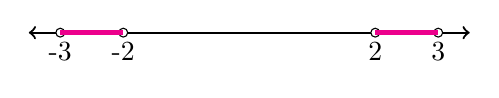
\begin{tikzpicture}[scale=0.8, baseline=0]
		% Number line
		\draw[thick, <->,] (-3.5,0) -- (3.5,0);
		% Interval
		\draw[fill=white] (2,0) circle (2pt);
		\draw[fill=white] (3,0) circle (2pt);
		\draw[fill=white] (-2,0) circle (2pt);
		\draw[fill=white] (-3,0) circle (2pt);
		\draw[-, magenta, ultra thick] (2,0) -- (3,0);
		\draw[-, magenta, ultra thick] (-2,0) -- (-3,0);
		\node at (2,-0.3) {2};
		\node at (3,-0.3) {3};
		\node at (-2,-0.3) {-2};
		\node at (-3,-0.3) {-3};
	\end{tikzpicture}
}
\def\tresiiiDos{
	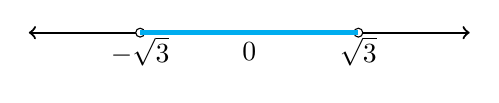
\begin{tikzpicture}[scale=0.8, baseline=0]
		% Number line
		\draw[thick, <->,] (-3.5,0) -- (3.5,0);
		% Interval
		\draw[fill=white] (1.732,0) circle (2pt);
		\draw[fill=white] (-1.732,0) circle (2pt);
		\draw[-, cyan, ultra thick] (1.732,0) -- (-1.732,0);
		\node at (1.732,-0.3) {$\sqrt{3}$};
		\node at (-1.732,-0.3) {$-\sqrt{3}$};
		\node at (0,-0.3) {0};
	\end{tikzpicture}
}

%12
\def\doceiA{
	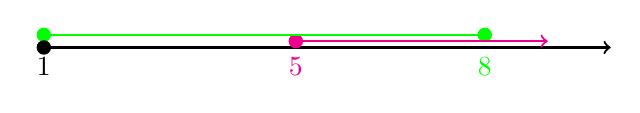
\begin{tikzpicture}[scale=0.8, baseline=0]
		% Number line
		\draw[thick, ->,] (1,0) -- (10,0);
		% Interval
		\draw[fill=magenta, color=magenta] (5,0.1) circle (3pt);
		\draw[fill=green, color=green] (8,0.2) circle (3pt);
		\draw[fill=green, color=green] (1,0.2) circle (3pt);
		\draw[fill=black] (1,0) circle (3pt);
		\draw[-, green, thick] (1,0.2) -- (8,0.2);
		\draw[->, magenta, thick] (5,0.1) -- (9,0.1);
		\node at (1,-0.3) {1};
		\node [color=magenta]at (5,-0.3) {5};
		\node[color=green] at (8,-0.3) {8};
	\end{tikzpicture}
}
\def\doceiiA{
	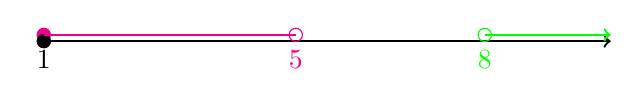
\begin{tikzpicture}[scale=0.8, baseline=0]
		% Number line
		\draw[thick, ->,] (1,0) -- (10,0);
		% Interval
		\draw[color=magenta] (5,0.1) circle (3pt);
		\draw[color=green] (8,0.1) circle (3pt);
		\draw[fill=magenta, color=magenta] (1,0.1) circle (3pt);
		\draw[fill=black] (1,0) circle (3pt);
		\draw[-, magenta, thick] (1,0.1) -- (5,0.1);
		\draw[->, green, thick] (8,0.1) -- (10,0.1);
		\node at (1,-0.3) {1};
		\node [color=magenta]at (5,-0.3) {5};
		\node[color=green] at (8,-0.3) {8};
	\end{tikzpicture}
}

\def\doceiiE{
	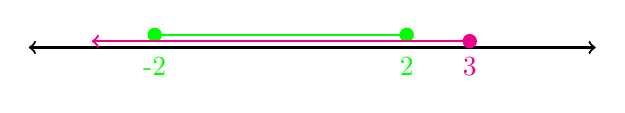
\begin{tikzpicture}[scale=0.8, baseline=0]
		% Number line
		\draw[thick, <->,] (-4,0) -- (5,0);
		% Interval
		\draw[fill=magenta, color=magenta] (3,0.1) circle (3pt);
		\draw[fill=green, color=green] (2,0.2) circle (3pt);
		\draw[fill=green, color=green] (-2,0.2) circle (3pt);
		\draw[<-, magenta, thick] (-3,0.1) -- (3,0.1);
		\draw[-, green, thick] (-2,0.2) -- (2,0.2);
		\node [color=magenta] at (3,-0.3) {3};
		\node[color=green] at (2,-0.3) {2};
		\node[color=green] at (-2,-0.3) {-2};
	\end{tikzpicture}
}

\def\doceiiicero{
	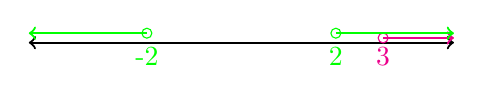
\begin{tikzpicture}[scale=0.6, baseline=0]
		% Number line
		\draw[thick, <->,] (-4.5,0) -- (4.5,0);
		% Interval
		\draw[color=magenta] (3,0.1) circle (3pt);
		\draw[color=green] (2,0.2) circle (3pt);
		\draw[color=green] (-2,0.2) circle (3pt);

		\draw[->, magenta, thick] (3,0.1) -- (4.5,0.1);
		\draw[<-, green, thick] (-4.5,0.2) -- (-2,0.2);
		\draw[->, green, thick] (2,0.2) -- (4.5,0.2);

		\node[color=magenta] at (3,-0.3) {3};
		\node[color=green] at (2,-0.3) {2};
		\node[color=green] at (-2,-0.3) {-2};
	\end{tikzpicture}
}

\def\doceiiiuno{
	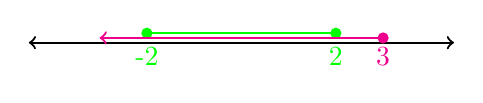
\begin{tikzpicture}[scale=0.6, baseline=0]
		% Number line
		\draw[thick, <->,] (-4.5,0) -- (4.5,0);
		% Interval
		\draw[fill=magenta, color=magenta] (3,0.1) circle (3pt);
		\draw[fill=green, color=green] (2,0.2) circle (3pt);
		\draw[fill=green, color=green] (-2,0.2) circle (3pt);

		\draw[<-, magenta, thick] (-3,0.1) -- (3,0.1);
		\draw[-, green, thick] (-2,0.2) -- (2,0.2);

		\node[color=magenta] at (3,-0.3) {3};
		\node[color=green] at (2,-0.3) {2};
		\node[color=green] at (-2,-0.3) {-2};
	\end{tikzpicture}
}

\def\doceiiidos{
	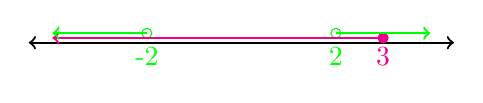
\begin{tikzpicture}[scale=0.6, baseline=0]
		% Number line
		\draw[thick, <->,] (-4.5,0) -- (4.5,0);
		% Interval
		\draw[fill=magenta, color=magenta] (3,0.1) circle (3pt);
		\draw[color=green] (2,0.2) circle (3pt);
		\draw[color=green] (-2,0.2) circle (3pt);

		\draw[<-, magenta, thick] (-4,0.1) -- (3,0.1);
		\draw[<-, green, thick] (-4,0.2) -- (-2,0.2);
		\draw[->, green, thick] (2,0.2) -- (4,0.2);

		\node[color=magenta] at (3,-0.3) {3};
		\node[color=green] at (2,-0.3) {2};
		\node[color=green] at (-2,-0.3) {-2};
	\end{tikzpicture}
}

\def\doceiiitres{
	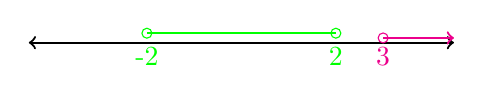
\begin{tikzpicture}[scale=0.6, baseline=0]
		% Number line
		\draw[thick, <->,] (-4.5,0) -- (4.5,0);
		% Interval
		\draw[color=magenta] (3,0.1) circle (3pt);
		\draw[color=green] (2,0.2) circle (3pt);
		\draw[color=green] (-2,0.2) circle (3pt);

		\draw[->, magenta, thick] (3,0.1) -- (4.5,0.1);
		\draw[-, green, thick] (-2,0.2) -- (2,0.2);

		\node[color=magenta] at (3,-0.3) {3};
		\node[color=green] at (2,-0.3) {2};
		\node[color=green] at (-2,-0.3) {-2};
	\end{tikzpicture}
}

% 17
\def\diecisietei{
	\begin{tikzpicture}[scale=0.5, >=Latex, draw=Aquamarine]
		%A vértices
		\node (1a) {$\bullet$};
		\node[] at (1a.west) {1};
		\node[below=of 1a] (2a) {$\bullet$};
		\node[] at (2a.west) {2};
		\node[below=of 2a] (3a) {$\bullet$};
		\node[] at (3a.west) {3};
		\node[shape=ellipse, draw, black, minimum size=2cm,fit={(1a) (3a)}] {};

		%B vértices
		\node[right=2cm of 1a] (1b) {$\bullet$};
		\node[] at (1b.east) {1};
		\node[below=of 1b] (3b) {$\bullet$};
		\node[] at (3b.east) {3};
		\node[below=of 3b] (5b) {$\bullet$};
		\node[] at (5b.east) {5};
		\node[below=of 5b] (7b) {$\bullet$};
		\node[] at (7b.east) {7};
		\node[shape=ellipse, draw, black, minimum size=2cm,fit={(1b) (7b)}] {};

		% Elipses
		\node[below=1cm of 3a] {$A$};
		\node[below=1.2cm of 7b] {$B$};

		% Aristas
		\draw[->, bend left] (1a) to (1b);
		\draw[->, bend right] (1a) to (3b);
		\draw[->, bend right] (1a) to (7b);
		\draw[->, bend right] (3a) to (1b);
		\draw[->, bend right] (3a) to (5b);
	\end{tikzpicture}
}

%19
\def\diecinuevei{
	\begin{tikzpicture}[scale=0.5, baseline=0, >=Latex, draw=Aquamarine]

		\node[] (a) {$\bullet$};
		\node[] at (a.west) {$a$};

		\node[above right= of a] (b) {$\bullet$};
		\node[] at (b.east) {$b$};

		\node[below right= of b] (c) {$\bullet$};
		\node[] at (c.east) {$c$};

		\node[below= of a] (d) {$\bullet$};
		\node[] at (d.west) {$d$};

		\node[below= of c] (e) {$\bullet$};
		\node[] at (e.west) {$e$};

		\node[right= of d] (f) {$\bullet$};
		\node[] at (f.west) {$f$};

		\node[right= of c] (g) {$\bullet$};
		\node[] at (g.north) {$g$};

		\node[below= of g] (h) {$\bullet$};
		\node[] at (h.south) {$h$};

		% Universo
		\node[shape=ellipse, draw, black, fit={ (b) (d) (g) (e)}] (universo) {};
		\node[above left = 0.1cm of universo] {$A$};

		% Aristas
		\draw[->, bend left] (a.center) to (b.center);
		\draw[->, bend left] (b.center) to (a.center);
		\draw[->, bend right] (c.center) to (d.center);
		\draw[->, loop above] (c) to (c);
		\draw[->, loop below ] (f) to (f);
		\draw[->, bend right] (c.center) to (h.center);
		\draw[->, bend left] (e.center) to (c.center);
		\draw[->, bend right] (h.center) to (g.center);
	\end{tikzpicture}
}

% 19 ii
\def\diecinueveiv{
	\begin{tikzpicture}[scale=0.5, baseline=0, >=Latex, draw=Aquamarine]

		\node[] (a) {$\bullet$};
		\node[] at (a.west) {$a$};

		\node[above right= of a] (b) {$\bullet$};
		\node[] at (b.east) {$b$};

		\node[below right= of b] (c) {$\bullet$};
		\node[] at (c.east) {$c$};

		\node[below= of a] (d) {$\bullet$};
		\node[] at (d.west) {$d$};

		\node[below= of c] (e) {$\bullet$};
		\node[] at (e.west) {$e$};

		\node[right= of d] (f) {$\bullet$};
		\node[] at (f.west) {$f$};

		\node[right= of c] (g) {$\bullet$};
		\node[] at (g.east) {$g$};

		\node[below= of g] (h) {$\bullet$};
		\node[] at (h.east) {$h$};

		% Universo
		\node[shape=ellipse, draw, black, fit={ (b) (d) (g) (e)}] (universo) {};
		\node[above left = 0.1cm of universo] {$A$};

		% Aristas
		\draw[->, loop below] (a) to (a);
		\draw[->, loop above ] (b) to (b);
		\draw[->, loop above] (c) to (c);
		\draw[->, loop below ] (d) to (d);
		\draw[->, loop below] (e) to (e);
		\draw[->, loop below] (f) to (f);
		\draw[->, loop above] (g) to (g);
		\draw[->, loop below ] (h) to (h);

		\draw[->, bend left] (a.center) to (b);
		\draw[->, bend left] (b.center) to (a);

		\draw[->, bend right] (e.center) to (h);
		\draw[->, bend right] (e.center) to (g);
		\draw[->, bend right] (h.center) to (g);
		\draw[->, bend right] (h.center) to (e);
		\draw[->, bend right] (g.center) to (h);
		\draw[->, bend right] (g.center) to (e);
	\end{tikzpicture}
}

%20

\def\veinte{
	\begin{tikzpicture}[scale=0.5, baseline=0, >=Latex, draw=Aquamarine]

		\node[] (1) {$\bullet$};
		\node[] at (1.west) {$1$};

		\node[above right= of 1] (2) {$\bullet$};
		\node[] at (2.east) {$2$};

		\node[below right= of 2] (3) {$\bullet$};
		\node[] at (3.east) {$3$};

		\node[below= of 1] (4) {$\bullet$};
		\node[] at (4.west) {$4$};

		\node[right= of 2] (5) {$\bullet$};
		\node[] at (5.west) {$5$};

		\node[right= of d] (6) {$\bullet$};
		\node[] at (6.east) {$6$};


		% Universo
		\node[shape=ellipse, draw, black, fit={ (1) (2) (3) (4)}] (universo) {};
		\node[above left = 0.1cm of universo] {$A$};

		% Aristas
		\draw[->, loop below] (1) to (1);
		\draw[->, loop above ] (3) to (3);
		\draw[->, loop above] (4) to (4);
		\draw[->, loop below ] (6) to (6);

		\draw[->, bend left] (6.center) to (4);
		\draw[->, bend left] (4.center) to (6);

		\draw[->, bend right] (1.center) to (3);
		\draw[->, bend right] (3.center) to (1);
	\end{tikzpicture}
}

%24
\def\veinticuatro{
	\begin{tikzpicture}[scale=0.5, baseline=0, >=Latex, draw=Aquamarine]

		\node[] (a) {$\bullet$};
		\node[] at (a.north west) {$a$};

		\node[below left = 1cm of a] (b) {$\bullet$};
		\node[] at (b.south) {$b$};

		\node[below right = 1cm of a] (f) {$\bullet$};
		\node[] at (f.south) {$f$};

		\node[above right = 1cm of a] (d) {$\bullet$};
		\node[] at (d.west) {$d$};

		\node[right=1cm of a] (c) {$\bullet$};
		\node[] at (c.south) {$c$};

		\node[right= of c] (e) {$\bullet$};
		\node[] at (e.south) {$e$};


		% Universo
    \node[shape=ellipse, draw, black, fit={ (a) (b) (d) (f) (e)}] (universo) {};
		\node[above left = 0.1cm of universo] {$A$};

		% Aristas
		\draw[->, loop above] (a) to (a);
		\draw[->, loop left ] (b) to (b);
		\draw[->, loop left] (c) to (c);
		\draw[->, loop above ] (d) to (d);
		\draw[->, loop right ] (e) to (e);
		\draw[->, loop right ] (f) to (f);

		\draw[->, bend left] (a.center) to (b);
		\draw[->, bend left] (b.center) to (a);
		\draw[->, bend left] (a.center) to (f);
		\draw[->, bend left] (f.center) to (a);
		\draw[->, bend left] (b.center) to (f);
		\draw[->, bend left] (f.center) to (b);

		\draw[->, bend right] (c.center) to (e);
		\draw[->, bend right] (e.center) to (c);
	\end{tikzpicture}
}

%25
\def\veintisiete{
	\begin{tikzpicture}[scale=0.5, baseline=0, >=Latex, draw=Aquamarine]

		\node[] (1) {$\bullet$};
		\node[] at (1.west) {$1$};

		\node[right = of 1] (92) {$\bullet$};
		\node[] at (92.east) {$92$};

		\node[below = of 1] (2) {$\bullet$};
		\node[] at (2.west) {$2$};

		\node[right = of 2] (91) {$\bullet$};
		\node[] at (91.east) {$91$};

		\node[below right = .5 of 2] (puntos) {$\vdots$};

		\node[below left = .5 of puntos] (45) {$\bullet$};
		\node[] at (45.west) {$45$};

		\node[right = of 45] (47) {$\bullet$};
		\node[] at (47.east) {$47$};


		\node[below right =.5 of 45] (46) {$\bullet$};
		\node[] at (46.east) {$46$};


		% Universo
    \node[shape=ellipse, draw, black, fit={ (1) (92) (45) (47) (46)}] (universo) {};
		\node[above left = 0.1cm of universo] {$A$};

		% Aristas
		\draw[->, loop below] (1) to (1);
		\draw[->, loop below ] (92) to (92);

		\draw[->, loop below] (2) to (2);
		\draw[->, loop below ] (91) to (91);

		\draw[->, loop below] (45) to (45);
		\draw[->, loop below ] (47) to (47);

		\draw[->, loop below ] (46) to (46);

		\draw[->, bend left] (1.center) to (92);
		\draw[->, bend left] (92.center) to (1);
		\draw[->, bend left] (2.center) to (91);
		\draw[->, bend left] (91.center) to (2);
		\draw[->, bend left] (45.center) to (47);
		\draw[->, bend left] (47.center) to (45);
	\end{tikzpicture}
}
